\section{Evaluating the performance of the proposed method}
\label{sec:rul_eval}

In this section we evaluate the performance of the proposed method. The architecture of the \gls{mlp} to be used here was presented in Section \ref{sec:method} Table \ref{table:proposed_nn} and will be used throughout this section.  The \gls{mlp} was trained $10$ times for$200$ epochs each and tested in each subset of the \gls{cmaps} dataset.

For the first experiment the combinations of window size $n_w$, window stride $n_s$ and early \gls{rul} $R_e$ presented in Table \ref{table:data_params_de} were tested obtaining the results shown in Table \ref{table:results_ann_de}.

\begin{table}[!htb]
\centering
\begin{tabular}{l l l l l}
	\hline
	 Dataset & Window Size $n_w$ & Window Stride $n_s$ & Early RUL $R_e$\\
  	\hline
  	FD001 & 30 & 2 & 120\\
  	FD002 & 20 & 2 & 120\\
  	FD003 & 30 & 2 & 120\\
  	FD004 & 18 & 2 & 120\\
  	\hline
\end{tabular}
\caption{Data-related parameters for each subset as obtained by \gls{de}.}
\label{table:data_params_de}
\end{table}  

\begin{table}[!htb]
\centering

\begin{tabular}{l | r r r r | r r r r}
	\hline	
	& \multicolumn{4}{| c}{RMSE} & \multicolumn{4}{| c}{RHS} \\
	Data Subset & Min. & Max. & Avg. & STD & Min. & Max. & Avg. & STD\\
  	\hline
  	FD001 & 14.78 & 15.25 & 14.98 & 0.13 & 3.41 & 4.40 & 3.94 & 0.30\\
  	FD002 & 29.76 & 31.55 & 30.67 & 0.50 & 59.25 & 95.36 & 69.25 & 10.68\\
  	FD003 & 15.05 & 16.05 & 15.54 & 0.33 & 3.24 & 4.98 & 3.86 & 0.57\\
  	FD004 & 34.61 & 37.75 & 35.58 & 0.99 & 55.46 & 91.94 & 69.06 & 11.12\\
  	\hline
\end{tabular}

\caption{Scores for each dataset using the data-related parameters obtained by \gls{de}.}
\label{table:results_ann_de}
\end{table}

Next, the possibility of using a single set of data-related parameters for all the subsets is explored. For this experiment the window size $n_w$ is fixed for all of the four datasets, given that the maximum allowable window size for all datasets is $18$, $n_w = 18$ will be used as window size throughout the four subsets. Details of the data-related chosen parameters are presented in Table \ref{table:data_params_1}, the results obtained are shown in Table \ref{table:results_ann_1}. 

\begin{table}[!htb]
\centering
\begin{tabular}{l l l l l}
	\hline
	 Dataset & Window Size $n_w$ & Window Stride $n_s$ & Early RUL $R_e$\\
  	\hline
  	All & 18 & 2 & 120\\
  	\hline
\end{tabular}
\caption{Single set of data-related parameters for all subsets.}
\label{table:data_params_1}
\end{table}  

\begin{table}[!htb]
\centering
\begin{tabular}{l | r r r r | r r r r}
	\hline	
	& \multicolumn{4}{| c}{RMSE} & \multicolumn{4}{| c}{RHS} \\
	Data Subset & Min. & Max. & Avg. & STD & Min. & Max. & Avg. & STD\\
  	\hline
  	FD001 & 17.45 & 19.29 & 18.12 & 0.63 & 6.60 & 8.96 & 7.45 & 0.81\\
  	FD002 & 29.64 & 31.93 & 30.28 & 0.67 & 49.02 & 95.62 & 60.65 & 14.18\\
  	FD003 & 15.90 & 16.80 & 16.19 & 0.32 & 3.63 & 5.11 & 4.04 & 0.45\\
  	FD004 & 33.63 & 36.43 & 34.63 & 0.86 & 52.14 & 78.47 & 61.87 & 8.47\\
  	\hline
\end{tabular}
\caption{Scores for each dataset using the single set of data-related parameters.}
\label{table:results_ann_1}
\end{table}

\pagebreak

As can be observed, performance is decreased for subsets FD001/FD003, this indicates that larger window sizes are beneficial for this regression problem. Figures \ref{fig:scores_rmse} and \ref{fig:scores_rhs} show a comparison of how the scores are affected for each dataset by changing the data-related parameters to make use of 2 and 1 sets of them.

\begin{figure}[!htb]
\centering
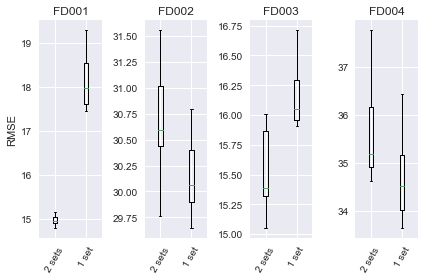
\includegraphics[width=0.5\textwidth]{img/rmse_comparisson.png}
\caption{Comparison of \gls{rmse} results for different sets of data-related parameters.}
\label{fig:scores_rmse}
\end{figure}

\begin{figure}[!htb]
\centering
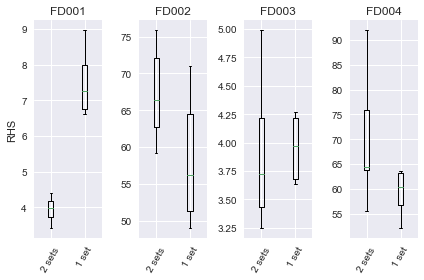
\includegraphics[width=0.5\textwidth]{img/rhs_comparisson.png}
\caption{Comparison of \gls{rhs} results for different sets of data-related parameters.}
\label{fig:scores_rhs}
\end{figure}